\section{Software and Hardware Design Implementation}
In order to allow for easier future interaction, a command system was introduced. The MCU receives commands over UART as a string with the format: \texttt{<command>, <value>}. These commands are interpreted by the MCU, changing the appropriate values.

\begin{center}
    \begin{tblr}{colspec={X[c]|X[c]}, width=0.9\linewidth}
        \hline
        Command     &   Value Changed   \\
        \hline 
        0           &   Change P        \\
        1           &   Change I        \\
        2           &   Change D        \\
        3           &   Change Setpoint \\
        4           &   Change Disturbance Value \\
        5           &   Change Duty Cycle  \\
        6           &   Change PWM Output   \\
        7           &   Change Start Flag\\
        \hline
    \end{tblr}
\end{center}

If the start variable is set, then the sampling process begins. First a timer is started, the PWM output flags variable is then checked to see which PWM signals must be set, and finally the samples are taken.

The samples are converted to temperatures using the temperature calibration equation. A running average of 200 samples is used to filer high frequency noise. The timer started at the beginning of the sampling process is then checked to see if the sampling period has passed, and if not, it waits for the remaining time.
The processed samples are again sent over UART as a string with the format:

\texttt{<Temp1>, <Temp2>, <PWM1>, <PWM2>, <Time>, <Message>}


The \texttt{<Message>} paramater is used to signal error data. Currently the only error message implemented is for if the sampling process takes longer than the set sampling period. (Currently $200~\mathrm{Hz}$)

\begin{figure}
    \centering
    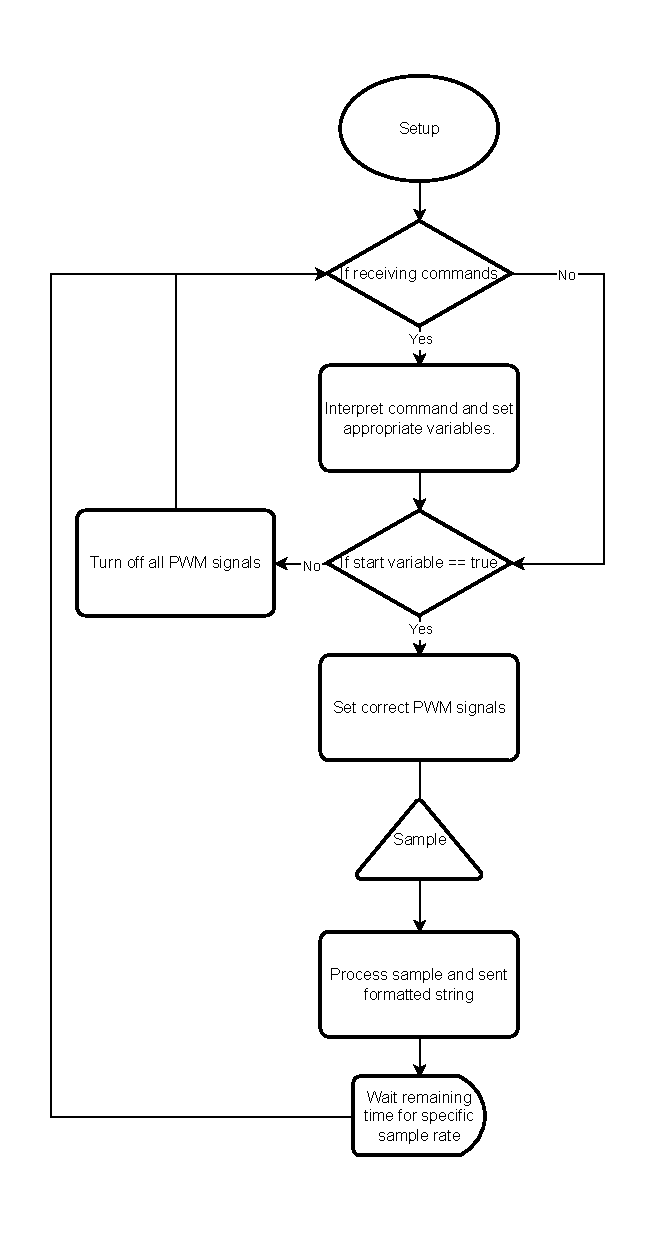
\includegraphics{Images/MCU_Flow1.drawio.pdf}
    \caption{Flow Diagram of MCU Code.}
    \label{fig:MCU_Flow1}
\end{figure}
\pagebreak

\begin{figure}
    \centering
    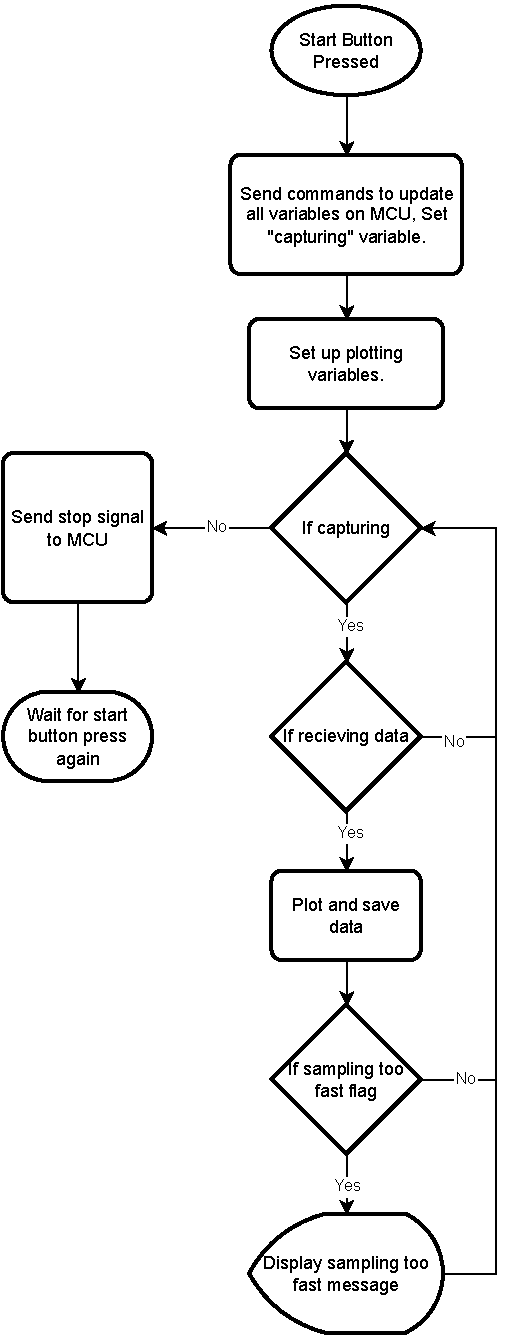
\includegraphics{Images/Matlab_Flow1.drawio.pdf}
    \caption{Flow Diagram of Matlab Code.}
    \label{fig:Matlab_Flow1}
\end{figure}
\pagebreak